\documentclass[a4paper,10pt]{article}
\usepackage{graphicx}



%opening
\title{Ticket 23: Support for RSP taggin}
\author{Group 3 - Jonathan Velasco}

\begin{document}

\maketitle

\begin{abstract}

Matthew said RSP uses their naming convention for files, internally.  This is a general ticket on how files should be tagged.  A couple of suggestions is to use key-values pairs as metadata  (minutes 20 March 2008)

\end{abstract}

\section{Design}

In order to address this ticket, some extra columns had been added to the 'file' table in the database.  See figure \ref{fig:filetable}

The column added are 'job', 'sequence' and 'shot'.  Each file in RSP will be under a specific directory structure, therefore, the information related to the 'job', 'sequence' and 'shot' is extracted from the path of such file.

\begin{figure}[h]
 \centering
 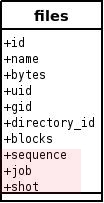
\includegraphics[scale=0.5]{images/fileTableModified.jpg}
 % fileTableModified.jpg: 1179666x1179666 pixel, 0dpi, infxinf cm, bb=
 \caption{New 'file' table}
 \label{fig:filetable}
\end{figure}

\section{Modifications Done}

\begin{itemize}
 \item In order to include the extra columns 'job', 'sequence' and 'shot' in the 'file' table, the file \textit{earth/db/migrate/060\_add\_rsp\_tag\_to\_files.rb} had been created.  See figure \ref{fig:columns}.  This task took aprox 30 minutes
\begin{figure}[h]
 \centering
 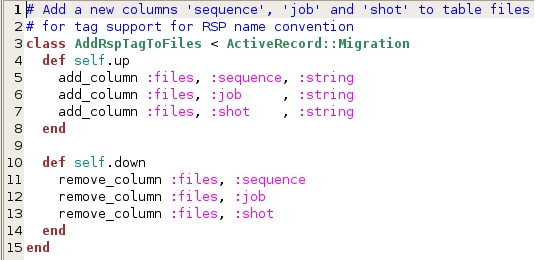
\includegraphics[scale=0.5]{images/060AddRspTagToFiles.jpg}
 % 060AddRspTagToFiles.jpg: 1179666x1179666 pixel, 0dpi, infxinf cm, bb=
 \caption{File to add the extra columns into the 'file' table}
 \label{fig:columns}
\end{figure}

\item In order to allow the user to search through 'job', 'sequence' and/or 'shot', the file \textit{earth/app/views/browser/\_breadcrumb\_and\_filter.html.haml }was modified as showed in figure \ref{fig:bread}. This changes are reflected in figure \ref{fig:earth}.  This took aprox 30 minutes
\begin{figure}[h]
 \centering
 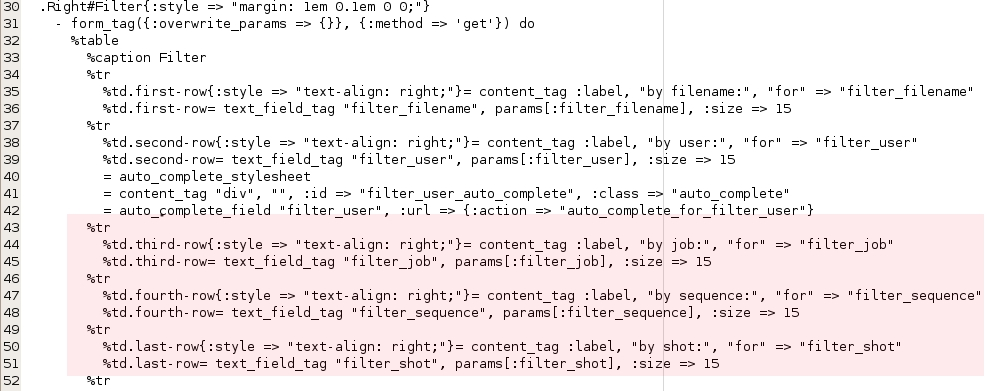
\includegraphics[scale=0.4]{images/bread.jpg}
 % bread.jpg: 1179666x1179666 pixel, 0dpi, infxinf cm, bb=
 \caption{Modifications to allow the user to search by 'job', 'sequence' and or 'shot'}
 \label{fig:bread}
\end{figure}
\begin{figure}[h]
 \centering
 
\includegraphics[scale=0.5]{images/earth.jpg}
 % earth.jpg: 1179666x1179666 pixel, 0dpi, infxinf cm, bb=
 \caption{Incorporation of extra fields for searching by RSP directory structure convention}
 \label{fig:earth}
\end{figure}

\item In order to populate the new columns in the 'file' table, some changes in \textit{earth/lib/earth\_plugins/file\_monitor.rb }where done as show in figure \ref{fig:monitor}.  The time expended in order to understand which file to change and how to do it was aprox 7 hours.  After finding  where the changes should be done, the time coding was aprox 10 minutes
\begin{figure}[h]
 \centering
 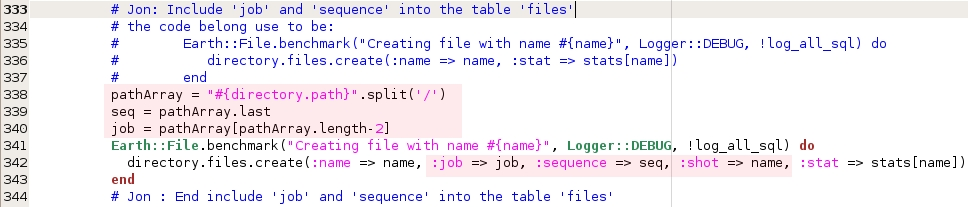
\includegraphics[scale=0.4]{images/monitor.jpg}
 % monitor.jpg: 1179666x1179666 pixel, 0dpi, infxinf cm, bb=
 \caption{Changes done to file\_monitor.rb}
 \label{fig:monitor}
\end{figure}

\item In order to execute the search, some lines were added to the file \textit{earth/app/models/earth/file.rb} in order to return only the files matching the searching criteria of the user.  See figure \ref{fig:file}.  This took aprox 20 minutes
\begin{figure}[h]
 \centering
 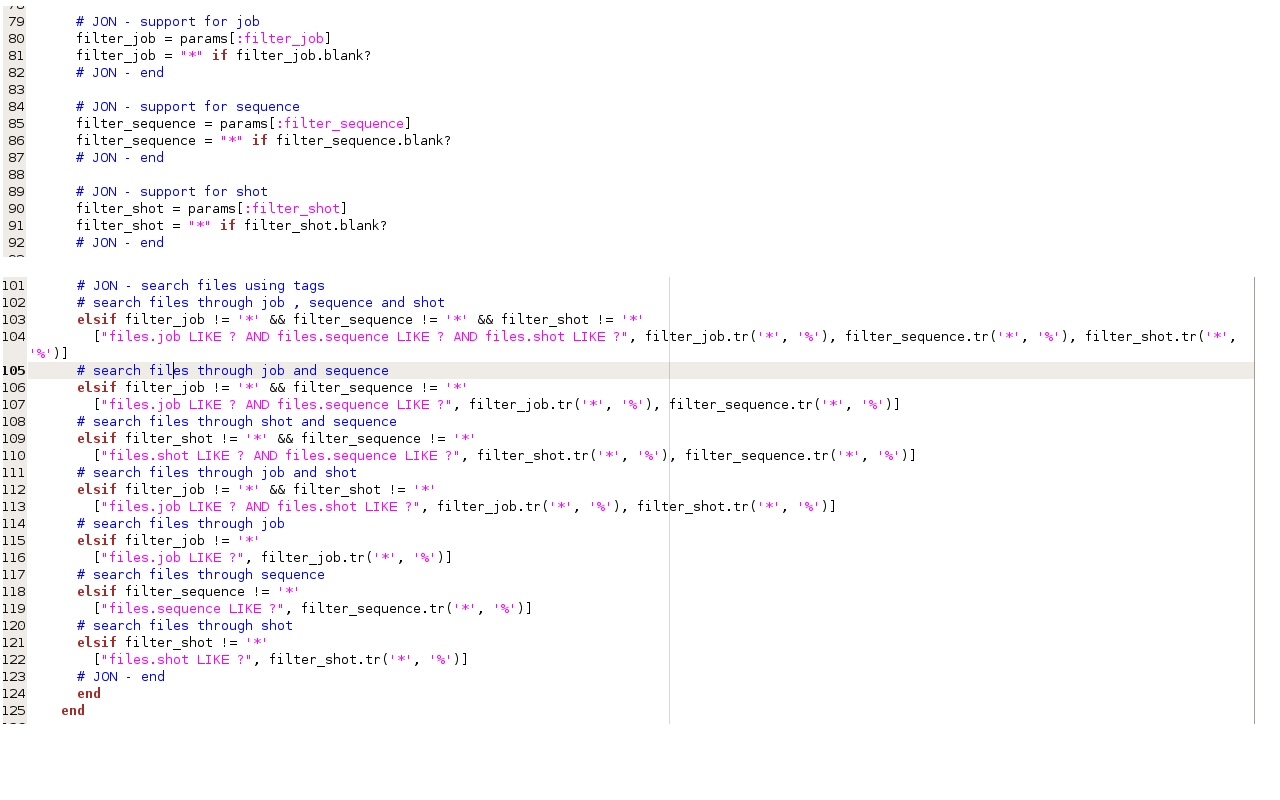
\includegraphics[scale=0.35]{images/file.jpg}
 % file.jpg: 1179666x1179666 pixel, 0dpi, infxinf cm, bb=
 \caption{Changes made to the file model}
 \label{fig:file}
\end{figure}


\end{itemize}






\end{document}
